% siminos/presentations/KITP17/UCSB17.tex        pdflatex UCSB17
% $Author: predrag $ $Date: 2017-02-13 03:48:01 -0500 (Mon, 13 Feb 2017) $

%  started with siminos/presentations/Israel16/Israel16.tex 2016-08-17
%  started with siminos/presentations/GTmap16/GTmap16.tex   2016-08-17
%  started with talks/predrag/NBI16/NBI16.tex               2016-04-25
%  started with talks/predrag/RoySoc16/RoySoc16.tex         2016-04-25

\input ../../inputs/layoutBeamer
\input ../../inputs/def % no edits, always from dasbuch/book/inputs
\input ../../inputs/defsBeamer
\renewcommand{\Ssym}[1]{{\ensuremath{m_{#1}}}}    % Boris
% \newcommand{\Ssym}[1]{{\ensuremath{s_{#1}}}}  % ChaosBook

\begin{document}


\title{
{\huge is space time?}
    \\
{a spatio-temporal theory of transitional turbulence}
}
\author{P. Cvitanovi\'c}
\author[Cvitanovi\'c]
{
  \textcolor{green!50!black}{
  {Predrag~Cvitanovi\'c \\
  Matt Gudorf,
  Nazmi Burak Budanur,
        Li Han,
        Rana Jafari,
		Adrien K. Saremi,
  and
  Boris Gutkin
  }	%\inst{1}
  }
}
\institute
{
%  \inst{1}%
Mathematics Colloquium
\\
                UC Santa Barbara
 }
\date{January 26, 2017}

\begin{frame}
  \titlepage
\end{frame}


\section[what this talk is about]
 {what this talk is about}

\begin{frame}{overview}
\begin{enumerate}
              \item {\Large
what this talk is about
                  }\textcolor{gray}{\small
              \item
``turbulence'' in small domains
              \item
coupled cat maps lattice
              \item
space is time
              \item
bye bye, dynamics
                    }
            \end{enumerate}
\end{frame}

\begin{frame}{The Day Dynamics Died}

\begin{block}{}
\centerline{\Huge R. I. P.}

\bigskip

\centerline{January 24, 2016 at 6 AM PST, Santa Barbara, CA}
\end{block}


\vfill\hfill why did it have to die?
\end{frame}

\begin{frame}{do clouds solve PDEs?}

%and do they care what PST hour is it?
%\\
%and at what longitude are they?
%\\
do clouds integrate Navier-Stokes equations?

\begin{center}
\centerline{\textcolor{red}{\Huge NO!}}
%\end{center}
%for weather prediction, we store sets of weather sequences
%\bigskip\bigskip

%\begin{center}
\begin{minipage}[t]{\textwidth}
	\begin{center}
%\vspace{2ex}
\centerline{
\raisebox{-4.0ex}[5.5ex][4.5ex]
		 {\includegraphics[height=12ex]{Hopf-a}}
~~~ $\Longrightarrow$ ~~ {other swirls} ~~ $\Longrightarrow$ ~~~
	\raisebox{-4.0ex}[5.5ex][4.5ex]
		 {\includegraphics[height=12ex]{Hopf-b}}
          }
	\end{center}
\end{minipage}
\end{center}

do clouds satisfy Navier-Stokes equations?

\bigskip

{\Large yes!}

\centerline{
\textcolor{blue}{they satisfy them \textcolor{red}{\large locally}, everywhere and at all times}
}
\end{frame}

\begin{frame}{part 1}
\begin{enumerate}
              \item {\Large
``turbulence'' in small domains
                  }\textcolor{gray}{\small
              \item
coupled cat maps lattice
              \item
space is time
              \item
bye bye, dynamics
                    }
            \end{enumerate}
\end{frame}


\begin{frame}{goal : go from equations to turbulence}
\begin{block}{Navier-Stokes equations} % (1822)}
\[
\dfrac{\partial \bv}{\partial t} + (\bv \cdot \nabla) \bv
	\,=\,
\frac{1}{R} \nabla ^2 \bv
-\nabla p
+ \mathbf{f}
    \,,\qquad
\nabla \cdot \bv = 0,
\]
\end{block}

\hfill{\small
velocity field  $\bv \in \mathbb{R}^3$
;
pressure field $p$
;
driving force $\mathbf{f}$
        }

\medskip

\begin{block}{describe turbulence}
starting from the equations (no statistical assumptions)
\end{block}

\bigskip

% large Reynolds number $R$:
\hfill {\Large\textcolor{red}{}}

\end{frame}

\begin{frame}{pipe experiment}
\begin{center}
\includegraphics[width=0.9\textwidth]{mullin_puff2200} %pipe}
\end{center}
T. Mullin lab
\end{frame}

\begin{frame}{example : pipe flow}
amazing data! amazing numerics!
\begin{center}
  \includegraphics[width=1.0\textwidth,clip=true]
                    {pipeSects}
\end{center}

%\begin{itemize}
% \item here each instant of the flow $\approx$ 2.5\,MB
% \item videos of the flow $\approx$ GBs
%\end{itemize}
\end{frame}

\section[dynamics in $\infty$ dimensions]
{dynamics in $\infty$ dimensions}

\begin{frame}{dynamical description of turbulence}
%	from {../chapter/dynsysII}

\begin{block}{\statesp}
a manifold $\pS \in \reals^{d}$ :
$d$ numbers determine the state of the system
\end{block}

\bigskip

\begin{block}{representative point }
$\ssp(t) \in \pS$
\\
a state of physical system at instant in time
\end{block}

\bigskip

\begin{block}{integrate the equations}
trajectory $\ssp(\zeit) = \flow{\zeit}{\xInit}$ =
representative point time $\zeit$ later
\end{block}
\end{frame}

\begin{frame}{charting the state space of a turbulent flow}

\begin{quote}{\scriptsize
  A long long time ago\\
I can still remember how\\
That dynamics used to make me smile\\
And I knew if I had my chance\\
That I could make those coherent structures dance\\
And maybe they'd be happy for a while
            }
\end{quote}

\vfill

John F Gibson (U New Hampshire)
\\
Jonathan Halcrow (Google)
\\
P. C. (Georgia Tech)
\end{frame}

\begin{frame}{plane Couette : so far, {\Huge small} computational cells}
\begin{center}
\includegraphics[width=0.5\textwidth]{statseSpProj3center}
\end{center}
velocity field visualization
\end{frame}

\begin{frame}{can visualize 61,506 dimensional \statesp\ of turbulent flow}
\begin{center}
\includegraphics[width=0.80\textwidth]{NCC1701b}
\end{center}
\eqva\ of turbulent plane Couette flow,
\\
their unstable manifolds, and
\\
myriad of turbulent videos mapped out as one happy family

\bigskip

\hfill   {\small
          for movies, please click through
            \textcolor{blue}{\href{http://ChaosBook.org/tutorials}
             {ChaosBook.org/tutorials}}
          }
\end{frame}

\begin{frame}{plane Couette state space $10^5 \to 3D$}
\begin{center}
\includegraphics[width=0.7\textwidth]{a1_14_g2}
\end{center}
\eqva, \po s, their (un)stable manifolds

\hfill   shape the turbulence
\end{frame}

\begin{frame}{part 2}
\begin{enumerate}
              \item
    \textcolor{gray}{\small
``turbulence'' in small domains
        }
              \item
    {\Large
coupled cat maps lattice
    }\textcolor{gray}{\small
              \item
space is time
              \item
bye bye, dynamics
                    }
            \end{enumerate}
\end{frame}

\begin{frame}{next: large space-time domains}
\begin{block}{example : complex Ginzburg-Landau on a large domain}
  \includegraphics[width=0.515\textwidth] %,height=0.5\textheight,clip=true]
  {cGLdefturbabs}
\end{block}

{\footnotesize
[horizontal] space $\ssp \in [-L/2,L/2]$
\qquad
{[up]} time evolution
}

\hfill {\scriptsize \color{orange} codeinthehole.com/static/tutorial/coherent.html}
\end{frame}

\begin{frame}{
describe $(\conf,\zeit) \in (-\infty, \infty)\times (-\infty, \infty)$
             }

\bigskip

continuous symmetries : space, time translations
\medskip

\begin{center}
\includegraphics[width=1.1\textwidth]{spaceTime}
\end{center}
% \hfill \color{red}{(impossible without xxx)}
\end{frame}

\begin{frame}{1) chaos and a single kitten}
\begin{center}
\includegraphics[width=1.05\textwidth]{Cat1200x800}
\end{center}
\end{frame}

\begin{frame}{example of a ``small domain dynamics'' : kicked rotor}
an electron circling an atom, subject to

a discrete time
sequence of angle-dependent kicks $F(x_{t})$

\hfill  \includegraphics[width=0.33\textwidth]{kicked-rotor}

\begin{block}{Taylor, Chirikov and Greene  standard map}
\bea
x_{t+1} &=& x_{t}+p_{t+1} \qquad  \mod 1, \continue
p_{t+1} &=& p_{t} + F(x_{t})             \nnu
\eea
\end{block}

\medskip

\hfill $\to$ {\color{red}
chaos in Hamiltonian systems}
\end{frame}

\begin{frame}{standard map}
\begin{block}{example of chaos in a Hamiltonian system}
  \includegraphics[width=0.515\textwidth] %,height=0.5\textheight,clip=true]
  {standard_k10}
\end{block}
\end{frame}

\begin{frame}{the simplest example : a single kitten in time}

force
\(
 F(x) = Kx
\)
linear in the displacement $x$
\,,\;
$K\in\integers$
\bea
x_{t+1} &=& x_{t}+p_{t+1} \quad  \mod 1
        \continue
p_{t+1} &=& p_{t} + K x_{t} \qquad  \mod 1 \nnu
\eea
 \textcolor{red}{C}ontinuous
 \textcolor{red}{A}utomorphism of the
 \textcolor{red}{T}orus, or

\begin{block}{Hamiltonian cat map}
a linear, area preserving map of a 2-torus onto itself
 \[
 \left(\begin{array}{c}
   x_{t+1}  \\
   p_{t+1}
  \end{array} \right )=
  A \left(\begin{array}{c}
   x_t  \\
   p_t
  \end{array} \right )\quad \mod 1
\,,\qquad
A = \left (
\begin{array}{cc}
s-1 & 1 \\
s-2 & 1 \\
\end{array}
    \right )
 \] %\ee{eq:CatMapIntr}
\end{block}
for integer
$s=\tr{A} > 2$ the map is hyperbolic $\to$ a
fully chaotic Hamiltonian dynamical system
\end{frame}

\begin{frame}{cat map in Lagrangian form}
replace momentum by velocity
\[
p_{t+1}=(\ssp_{t+1}  - \ssp_{t})/\Delta t
\]
dynamics in $(\ssp_{t},\ssp_{t-1})$  \statesp\
is particularly simple
\begin{block}{2-step difference equation}
\[
\ssp_{t+1}  -  s \, \ssp_{t} + \ssp_{t-1}
    =
-\Ssym{t}
\] %\ee{eq:CatMapNewton1}
\end{block}
unique integer $\Ssym{t}$
ensures that

\hfill $\ssp_{t}$ lands in the unit interval at every time step $t$

\bigskip
nonlinearity : $ \mod 1$ operation, encoded in
\[
\Ssym{t}\in  \A
\,,\quad \A\ = \mbox{ finite alphabet of possible values for } \Ssym{t}
\]
\end{frame}

\begin{frame}{example : $s=3$ cat map symbolic dynamics}
%%%%%%%%%%%%%%%%%%%%%%%%%%%%%%%%%%%%%%%%%%%%%%%%%%%%%%%%%%%%%%%%
%\begin{figure}
  \begin{center}  %%% 2016-12-25  see
                  %%% siminos/figsSrc/inkscape/CatMapStatesp.svg
  \setlength{\unitlength}{0.55\textwidth}
 %% \unitlength = units used in the Picture Environment
  \begin{picture}(1,0.81984366)%
    \put(0,0){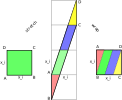
\includegraphics[width=\unitlength]{CatMapStatesp}}%
    \put(-0.025,0.15){\color[rgb]{0,0,0}\makebox(0,0)[lb]{\smash{}}}%
    \put(0.26669086,0.17307744){\color[rgb]{0,0,0}\makebox(0,0)[lb]{\smash{B}}}%
    \put(0.26669086,0.41839762){\color[rgb]{0,0,0}\makebox(0,0)[lb]{\smash{C}}}%
    \put(0.02137069,0.41839762){\color[rgb]{0,0,0}\makebox(0,0)[lb]{\smash{D}}}%
    \put(0.38935094,0.00135332){\color[rgb]{0,0,0}\makebox(0,0)[lb]{\smash{B}}}%
    %\put(0.32,0.17){\color[rgb]{0,0,0}\makebox(0,0)[lb]{\smash{$(0,0)$}}}%
    \put(0.64284833,0.60647641){\color[rgb]{0,0,0}\makebox(0,0)[lb]{\smash{C}}}%
    \put(0.64284833,0.79455521){\color[rgb]{0,0,0}\makebox(0,0)[lb]{\smash{D}}}%
    %\put(0.79004043,0.42657495){\color[rgb]{0,0,0}\makebox(0,0)[lb]{\smash{A}}}%
    %\put(0.79004043,0.17307744){\color[rgb]{0,0,0}\makebox(0,0)[lb]{\smash{B}}}%
    %\put(0.96994189,0.17307744){\color[rgb]{0,0,0}\makebox(0,0)[lb]{\smash{C}}}%
    %\put(0.97811923,0.42657495){\color[rgb]{0,0,0}\makebox(0,0)[lb]{\smash{D}}}%
    \put(0.02,0.27){\color[rgb]{0,0,0}\rotatebox{90.0}{\makebox(0,0)[lb]{\smash{$\ssp_{0}$}}}}%
    \put(0.39,0.27){\color[rgb]{0,0,0}\rotatebox{90.0}{\makebox(0,0)[lb]{\smash{$\ssp_{1}$}}}}%
    \put(0.76,0.27){\color[rgb]{0,0,0}\rotatebox{90.0}{\makebox(0,0)[lb]{\smash{$\ssp_{1}$}}}}%
    \put(0.1469525,0.16){\color[rgb]{0,0,0}\makebox(0,0)[lb]{\smash{$\ssp_{-1}$}}}%
    \put(0.51493279,0.16){\color[rgb]{0,0,0}\makebox(0,0)[lb]{\smash{$\ssp_{0}$}}}%
    \put(0.86655824,0.16){\color[rgb]{0,0,0}\makebox(0,0)[lb]{\smash{$\ssp_{0}$}}}%
    \put(0.21762677,0.55482852){\color[rgb]{0,0,0}\rotatebox{43.35476392}{\makebox(0,0)[lb]{\smash{stretch}}}}%
    \put(0.74915379,0.61465381){\color[rgb]{0,0,0}\rotatebox{-46.94301089}{\makebox(0,0)[lb]{\smash{wrap}}}}%
  \end{picture}%
\end{center}

%   \caption{ \label{fig:CatMapStatesp}
cat map stretches the unit square

translations by

\hfill $\Ssym{0} \in \A=\{\underline{1},0,1,2\}=$
\{%
{\color{red}red},
{\color{green}green},
{\color{blue}blue},
{\color{yellow}yellow}%
\}

return stray kittens back to the torus
%   }
% \end{figure}
\end{frame}

\begin{frame}{cat map $(\ssp_{0},\ssp_{1})$  \statesp\ partition}
%%%%%%%%%%%%%%%%%%%%%%%%%%%%%%%%%%%%%%%%%%%%%%%%%%%%%%%%%%%%%%%%%%
%\begin{figure}
\begin{center}
	\includegraphics[width=0.75\textwidth]{SingleCat1Symbol}
\end{center}
%	\caption{\label{fig:SingleCat1color}

{\scriptsize
(a) 4 regions labeled by $\Ssym{0}.$ , obtained from
$(\ssp_{-1},\ssp_{0})$ \statesp\ by one iteration
\\
(b) 14 regions, 2-steps past $\Ssym{-1}\Ssym{0}.$
(c) 44 regions, 3-steps past $\Ssym{-2}\Ssym{-1}\Ssym{0}.$

\medskip

(d) 4 regions labeled by future $.\Ssym{1}$
\\
(e) 14 regions, 2-steps  future $.\Ssym{1}\Ssym{2}$
(f) 44 regions, 3-steps future {\brick} $\Ssym{3}\Ssym{2}\Ssym{1}.$
}
%\end{figure}
%%%%%%%%%%%%%%%%%%%%%%%%%%%%%%%%%%%%%%%%%%%%%%%%%%%%%%%%%%%%%%%%%%
\end{frame}

\begin{frame}{2) chaos and the spatiotemporally infinite cat}
%\begin{center}
%\hfill\includegraphics[width=0.55\textwidth]{spatiotempCat}
\hfill\includegraphics[width=0.55\textwidth]{DawnBishopCats}
%\end{center}
\end{frame}


\begin{frame}{spatiotemporal cat map}
Consider
a 1\dmn\ spatial lattice, with field $\ssp_{n,t}$  (the angle of a kicked
rotor ``particle'' at instant $t$)  at site $n$.

\bigskip

require
\\
(0) each site couples to
its nearest neighbors $\ssp_{n\pm1,t}$
\\(1) invariance under
spatial translations
\\(2) invariance under spatial reflections
\\(3) invariance under the space-time exchange

\bigskip

obtain
\begin{block}{2\dmn\ coupled cat map lattice}
\[
\ssp_{n,t+1} + \ssp_{n,t-1} - s \, \ssp_{n,t} + \ssp_{n+1,t} + \ssp_{n-1, t}
     =-\Ssym{n,t}
\] %\ee{eq:CatMapNewton2}
\end{block}
\end{frame}

\begin{frame}{herding cats : a Euclidean field theory}
convert the spatial-temporal differences to discrete derivatives

\bigskip

discrete $d$\dmn\ Euclidean space-time Laplacian
in $d=1$ and $d=2$ dimensions

\bigskip

\(
\Box \ssp_t \;\;\,=\, \ssp_{t+1} - 2\ssp_{t} + \ssp_{t-1}
\)\\ \(
\Box \ssp_{n,t} \,=\, \ssp_{n,t+1} + \ssp_{n,t-1}
- 4 \, \ssp_{n,t} + \ssp_{n+1,t} + \ssp_{n-1, t}
\)

\medskip

$\to$ the cat map equations generalized  to
\begin{block}{$d$\dmn\ \catlatt}
\[
 (\Box -s+2d)\ssp_{z} = \m_z
%    \,, \qquad
\] %\ee{LinearConn}

\medskip

\end{block}

\bigskip

where
\(
  \ssp_{z} \in  \mathbb{T}^{1}
    \,, \quad
  \Ssym{z} \in \A
    \mbox{  and  }
  z\in \integers^{d}
\) = lattice site label
\end{frame}

\begin{frame}{deep insight, derived from observing kittens}
an insight that applies
to all coupled-map lattices, and all PDEs with translational symmetries

\bigskip

a $d$\dmn\ spatiotemporal pattern\\
\(
\{\ssp_{z}\} = \{\ssp_{z},  z\in \integers^{d}  \}
\)

\bigskip

is labelled by a \textcolor{red}{{\em $d$\dmn} spatiotemporal {\brick} of symbols}\\
\(
\{\m_{z}\} = \{\m_{z}, z\in \integers^{d}\}
\,,
\)

\bigskip

rather than a \textcolor{red}{single} temporal symbol sequence


\bigskip

(as is done
when describing a small coupled few-``particle'' system, or a small
computational domain).
\end{frame}


\begin{frame}{``\po s'' are now invariant $d$-tori}


\begin{block}{1 time, 0 space dimensions}
a {\statesp} point is {\em periodic} if its orbit returns to it
after a finite time \period{}; in time direction such orbit tiles the time axis
by infinitely many repeats
\end{block}

\bigskip

\begin{block}{1 time, $d$-1 space dimensions}
 a {\statesp} point is {\em spatiotemporally periodic} if
it belongs to an invariant $d$-torus ${\R}$, \ie, a \brick\ $\Mm_{\R}$ that
tiles the lattice state  $\Mm$ periodically, with period $\ell_j$ in
$j$th lattice direction
\end{block}
\end{frame}

\begin{frame}{an example of \twots\ : \\ shadowing, symbolic dynamics space}
%%%%%%%%%%%%%%%%%%%%%%%%%%%%%%%%%%%%%%%%%%%%%%%%%%%%%%%%%%%%%%%%%%%%%%%
%\begin{figure}
\begin{center}
\includegraphics[width=0.45\textwidth]
{AKSs7colrBorderM1}\hspace{0.7cm}\includegraphics[width=0.45\textwidth]
{AKSs7colrBorderM2}
%{AKSs7BlockBorderM1}\hspace{0.7cm}\includegraphics[width=0.45\textwidth]
%{AKSs7BlockBorderM2}
\end{center}
%\caption[]{
2d symbolic representation of two {\twots}
shadowing each other within the shared
\brick\ $\Mm_{\R}=\Mm_{\R_{0}} \cup \Mm_{\R_{1}}$ (blue)

\begin{itemize}
  \item border $\R_{1}$ (thick black), interior $\R_{0}$ (thin black)
  \item symbols outside \R\ differ
\end{itemize}

% for $s=7$.
%}
%\label{fig:AKScloseActSymb}
%\end{figure}
%%%%%%%%%%%%%%%%%%%%%%%%%%%%%%%%%%%%%%%%%%%%%%%%%%%%%%%%%%%%%%%%%%%%%%%
\end{frame}

\begin{frame}{shadowing, \statesp}
%%%%%%%%%%%%%%%%%%%%%%%%%%%%%%%%%%%%%%%%%%%%%%%%%%%%%%%%%%%%%%%%%%%%%%%
%\begin{figure}
\begin{center}
\includegraphics[width=0.40\textwidth]
{AKSs7BlockBorderG1}\hspace{0.7cm}\includegraphics[width=0.45\textwidth]
{AKSs7BlockBorderG2}
\end{center}
%\caption[]{
(left)  \statesp\ points $(\ssp_{0,t},\ssp_{0,t-1})$ of the two \twots\

(right) zoom into the small rectangular area

interior points $\in \R_{0}$ (large green), (small red) circles respectively

border points $\in \R_{1}$ (large violet), (small magenta)  squares respectively

within the interior of the shared \brick, the shadowing is exponentially small
%}
%\label{fig:AKScloseActSp}
%\end{figure}
%%%%%%%%%%%%%%%%%%%%%%%%%%%%%%%%%%%%%%%%%%%%%%%%%%%%%%%%%%%%%%%%%%%%%%%
\end{frame}

\begin{frame}{part 3}
\begin{enumerate}
              \item
    \textcolor{gray}{\small
``turbulence'' in small domains
              \item
coupled cat maps lattice
        }
              \item
    {\Large
space is time
    }\textcolor{gray}{\small
              \item
bye bye, dynamics
                    }
            \end{enumerate}
\end{frame}

\begin{frame}{yes, lattice schmatiz, but}
\begin{center}
{\huge does it work for PDEs?}
\end{center}
\end{frame}


\begin{frame}{chronotope}
\begin{bartlett}{
In literary theory and philosophy of language, the chronotope is how
configurations of time and space are represented in language and
discourse.
                }\bauthor{
\HREF{https://en.wikipedia.org/wiki/Chronotope}
{Wikipedia : Chronotope}
                }
\end{bartlett}

\bigskip
\bigskip
%goes without saying : was done by a Soviet scientist first

\begin{itemize}
  \item Mikhail Mikhailovich Bakhtin (1937)
  \item Politi, Giacomelli, Lepri, Torcini (1996)
%  \item Gutkin and Osipov (2016)
\end{itemize}
\end{frame}

\begin{frame}{space-time complex Ginzburg-Landau on a large domain}
\begin{block}{a nearly recurrent chronotope}
  \includegraphics[width=0.4635\textwidth]{cGLdefturbabs}%
~~\raisebox{+3.33ex}[5.5ex][4.5ex]
		 {\includegraphics[width=0.36\textwidth]{cGLdefturbclip}}
\end{block}

{\footnotesize
[horizontal] space $\ssp \in [-L/2,L/2]$
\qquad
{[up]} time evolution
}
\end{frame}

\begin{frame}{
must have : 2D symbolic dynamics
$\in (-\infty, \infty)\times (-\infty, \infty)$
             }
\begin{center}
\includegraphics[width=0.8\textwidth]{recurrence}
\end{center}
% \hfill \color{red}{(impossible without xxx)}

%\hfill Gutkin and Osipov (2016)
\end{frame}


\begin{frame}{(1+1) space-time dimensional ``Navier-Stokes''}
computationally not ready yet to explore the inertial manifold of
$(1+3)$\dmn\ turbulence - start instead with $(1+1)$\dmn\

\bigskip

\begin{block}{\KS\ time evolution equation}
\[
  u_t + u \triangledown u \,=\,
    {\color{red}-}\triangledown^2 u {\color{red}-\triangledown^4 u}
    \,,\qquad   x \in [-L/2,L/2]
    \,,
\]
\end{block}

\bigskip

describes spatially extended systems such as
\begin{itemize}
 \item flame fronts in combustion
 \item reaction-diffusion systems
 \item \ldots
\end{itemize}

\end{frame}

\begin{frame}{a test bed : \KS\ on a large domain}
\begin{center}
  \includegraphics[width=0.6\textwidth] %,height=0.5\textheight,clip=true]
  {ks_largeL_cbar_200} %{ksevol-fig} %{ks_largeL_cbar}
\end{center}

{\footnotesize
[horizontal] space $\ssp \in [0,L]$
\qquad
{[up]} time evolution
}

\begin{itemize}
\item turbulent behavior
\item simpler physical, mathematical and computational setting than Navier-Stokes
\end{itemize}
\end{frame}

\begin{frame}{compact space, infinite time cylinder}
\begin{center}
\includegraphics[width=0.9\textwidth]{cylinderTime}
\end{center}
% \hfill \color{red}{(impossible without xxx)}
so far : Navier-Stokes on compact spatial domains, all times
\end{frame}

\begin{frame}{compact space, infinite time \KS}

\begin{block}{in terms of discrete spatial Fourier modes}
$N$ ordinary differential equations (ODEs) in time
\[
\dot{\Fu}_k(\zeit) = ( q_k^2 - q_k^4 )\, \Fu_k(\zeit)
- i \frac{q_k}{2} \!\sum_{k'=0}^{N-1} \!\!\Fu_{k'}(\zeit) \Fu_{k-k'}(\zeit)
\,.
%\label{e-Fks}
\]
\end{block}
\end{frame}


\subsection{types of solutions}
\begin{frame}{evolution of \KS\ on small $L=22$ cell}
\begin{center}
  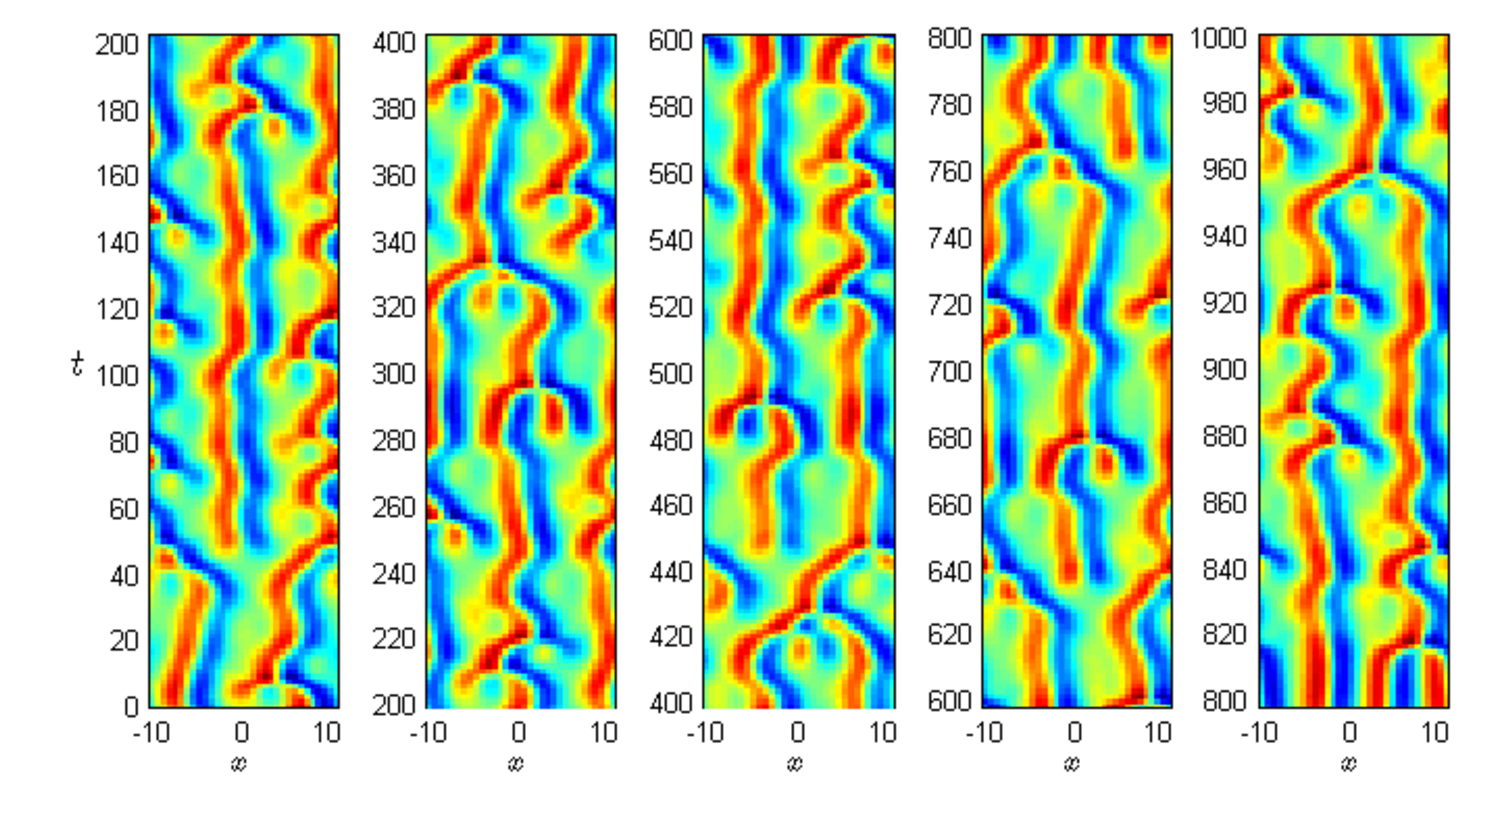
\includegraphics[width=0.9\textwidth,clip=true]{ks_L22_long_orbit}
\end{center}
horizontal: $x \in [-11,11]$
\\
vertical: time
\\
color: magnitude of $u(x,t)$
\end{frame}

\begin{frame}{yes, but}
\begin{center}
{\huge is space time?}
\end{center}
\end{frame}

\begin{frame}{compact time, infinite space cylinder}
\begin{center}
\includegraphics[width=0.9\textwidth]{cylinderSpace}
\end{center}
% \hfill \color{red}{(impossible without xxx)}
\end{frame}

\begin{frame}{compact time, infinite space \KS}
\bea
    u_\zeit &=&  - u u_\conf
    -u_{\conf \conf}-u_{\conf \conf \conf \conf}\,,
    % \label{e-ks}
\continue
    u^{(0)} &\equiv& u \, , \quad
    u^{(1)} \equiv u_{\conf} \, , \quad
    u^{(2)} \equiv u_{\conf \conf} \, , \quad
    u^{(3)} \equiv u_{\conf \conf \conf}
                        \nonumber
\eea
\begin{block}{periodic boundary condition in time
              $u(\conf, \zeit) = u(\conf, \zeit + \period{})$}
evolve $u(\zeit, \conf)$ in $\conf$,
4 equations, 1st order in spatial
derivatives
\bea
    u^{(0)}_{\conf} &=& u^{(1)} \,,\quad
    u^{(1)}_{\conf}  =  u^{(2)} \,,\quad
    u^{(2)}_{\conf}  =  u^{(3)} \continue
    u^{(3)}_{\conf} &=& - u^{(0)}_{\zeit} - u^{(2)} - u^{(0)} u^{(1)}
                        \nonumber
\eea
\end{block}

\bigskip

initial values
$u( \conf_0, \zeit)$,
$u_{\conf}( \conf_0, \zeit)$,
$u_{\conf \conf}( \conf_0, \zeit)$,
$u_{\conf \conf \conf}( \conf_0, \zeit)$,
    \\
for all $\zeit \in [0, \period{})$ at a space point $\conf_0$
\end{frame}

\begin{frame}{a time-invariant \eqv, spatial \po}
\begin{center}
  \begin{minipage}[height=.45\textheight]{.45\textwidth}
    \centering \small{\texttt{(a)}}
    \includegraphics[width=\textwidth,height=.45\textheight]{MNGeq1time}
  \end{minipage}
  \begin{minipage}[height=.45\textheight]{.45\textwidth}
    \centering \small{\texttt{(b)}}
    \includegraphics[width=\textwidth,height=.45\textheight]{MNGeq1space}
  \end{minipage}
\end{center}
   %\caption{
  evolution of $\EQV{1}$ : (a) in time, (b) in space
   \\
   initial condition for the spatial integration is the time strip
   $u(\conf_0,\zeit)$, $\zeit = [0,\period{})$, where time period
   $\period{} =0$, spatial $x$ period is $L=22$.
   % }\label{fig:MNGeqva1spttmp}

\vfill\hfill        Michelson 1986
\end{frame}


\begin{frame}{chronotope : }

a finite $(1+D)$\dmn\ symbolic dynamics rectangle

\begin{center}
\includegraphics[width=0.8\textwidth]{recurrence}
\end{center}
\hfill \color{red}{make it doubly periodic}
\end{frame}

\begin{frame}{compact space and time chronotope}
\begin{center}
\includegraphics[width=0.9\textwidth]{torusSpTime}
\end{center}
% \hfill \color{red}{(impossible without xxx)}
\end{frame}

\begin{frame}{a spacetime \twot}
\begin{center}
  \begin{minipage}[height=.40\textheight]{.35\textwidth}
    \centering \small{\texttt{(a)}}
    \includegraphics[width=\textwidth,height=.60\textheight]{MNGcomp32xint22}
  \end{minipage}
~~~~~~~~~
  \begin{minipage}[height=.40\textheight]{.35\textwidth}
    \centering \small{\texttt{(b)}}
    \includegraphics[width=\textwidth,height=.60\textheight]{MNGcomp64xint22}
  \end{minipage}
\end{center}
    (a) old : time evolution. (b) new : space evolution
    \\
    $x=[0,L]$ %22]$,
       initial condition : time periodic line $t = [0,T]$
  %2\,T_{\PPO{10.2}})$
  %\label{fig:MNGcompxint2}

\vfill\hfill        Gudorf 2016
\end{frame}


%\section[dimension of the inertial manifold]
%{dimension of the inertial manifold}


\begin{frame}{zeta function for a field theory ? much like Ising model}
\begin{block}{"\po s" are now spacetime tilings}
\[
Z(s) \approx
\sum_{p} \frac{e^{-A_p s}}
              {\left|\det(1-J_p)\right|}
\]
tori / spacetime tilings :
each of area $A_p = L_p T_p$
\end{block}
\begin{block}{symbolic dynamics : $(1+D)$\dmn}
essential to encoded shadowing
\end{block}

\vfill
at this time : this zeta is still but a dream
\end{frame}

\begin{frame}{part 4}
\begin{enumerate}
              \item
    \textcolor{gray}{\small
``turbulence'' in small domains
              \item
coupled cat maps lattice
              \item
space is time
    }
              \item
    {\Large
bye bye, dynamics
    }
            \end{enumerate}
\end{frame}

\begin{frame}{computing spacetime solutions}
\begin{center}
\includegraphics[width=0.65\textwidth]{arrival}
\end{center}
\end{frame}

\begin{frame}{kiss your DNS codes}
\begin{center}
{\huge goodbye}
\end{center}

\vfill

for long time and/or space integrations

\medskip

\hfill they never worked and could never work
\end{frame}

\begin{frame}{life outside of time}
\textcolor{red}{the trouble}:

forward time-integration codes too unstable

\bigskip
\bigskip

\textcolor{blue}{multishooting inspiration}:
 replace a guess that a  \textcolor{blue}{point} is on the periodic
orbit by a guess of the \textcolor{blue}{entire orbit}.

\bigskip

\textcolor{blue}{an example is ``Newton descent''} :
a variational method
to drive the initial guess toward the exact solution.

\bigskip

$\to$

\bigskip

a variational method for finding
spatio-temporally periodic solutions of classical field theories
\end{frame}

\begin{frame}{compute locally, adjust globally}

Computing literature : parallelizing {\color{red}spatiotemporal}
computation is FLOPs intensive, but more robust than
integration forward in time

\end{frame}


\begin{frame}{$1d$ example : variational principle for any \po}
$N$ guess points \textcolor{red}{$\to$ $\infty$ points}
along a smooth loop
(snapshots of the pattern at successive time instants)%
\footnote{Y.~Lan and P.~Cvitanovic',
        ``Variational method for finding periodic orbits
        in a general flow,''
	{Phys. Rev. \bf E 69}, 016217 (2004);
         {\tt nlin.CD/0308008}.
	 }
\end{frame}

\begin{frame}{a guess loop vs. the desired solution}
\begin{center}
\begin{minipage}[c]{0.55\textwidth}
\begin{center}

	\vskip 1.5cm

loop \textcolor{blue}{defines}
tangent vector $\lVeloc$

	\vskip 3cm

periodic orbit \textcolor{blue}{defined} by
\\
velocity field $\pVeloc(\pSpace)$

\end{center}
\end{minipage}%
~~~~~~~\begin{minipage}[c]{0.40\textwidth}
	\begin{center}
	\vskip 10pt
	\includegraphics[width=0.65\textwidth]{loop}
	\vskip 1.5cm
	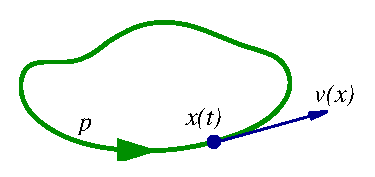
\includegraphics[width=0.72\textwidth]{porbit}
	\end{center}
\end{minipage}
\end{center}
\end{frame}


\begin{frame}{extremal principle for a general flow}
\begin{center}
\begin{minipage}[c]{0.55\textwidth}

	\vskip 10pt

\textcolor{red}{loop tangent}
$\lVeloc(\lSpace)
	\neq
\pVeloc(\lSpace)$

	\vskip 1cm

\textcolor{green}{periodic orbit}
$\lVeloc(\lSpace)$,~$\pVeloc(\lSpace)$
aligned
\end{minipage}%
~~~~~~~\begin{minipage}[c]{0.40\textwidth}
	\begin{center}
	\vskip 10pt
	\includegraphics[width=0.8\textwidth]{velocField}
	\end{center}
\end{minipage}
\end{center}

\begin{block}{cost function}%
\[
\costF[\lSpace] =
            \oint_\Loop ds\,(\lVeloc-\pVeloc)^2
    \,;\quad
    \lVeloc = \lVeloc(\lSpace(s,\tau))\,,\,\,
    \pVeloc = \pVeloc(\lSpace(s,\tau))
\,,
% \label{loopCostFct}
\]
\end{block}

\bigskip

penalizes misorientation of the loop tangent
$\lVeloc(\lSpace)$
relative to the true dynamical flow $\pVeloc(\lSpace)$
\end{frame}

\begin{frame}{Newton descent}
\bigskip

% \textcolor{blue}{Newton Descent}
cost minimization

\bigskip

\begin{center}
\begin{minipage}[c]{0.55\textwidth}
\begin{center}
\bigskip

drives

\bigskip

	\vskip 1.0cm

\textcolor{red}{initial guess $\Loop(0)$}
\\$\to$\\
\textcolor{green}{cycle $p = \Loop(\infty)$}

	\vskip 1.0cm

as fictitious time $\tau \to \infty$
\end{center}
\end{minipage}%
~~~~~~~\begin{minipage}[c]{0.40\textwidth}
	\begin{center}
	\includegraphics[width=0.7\textwidth]{tube}
	\end{center}
\end{minipage}
\end{center}
\end{frame}

\begin{frame}{clouds do not solve PDEs}

%and do they care what PST hour is it?
%\\
%and at what longitude are they?
%\\
do clouds integrate Navier-Stokes equations?

\begin{center}
\centerline{\textcolor{red}{\Huge NO!}}
%\end{center}
%for weather prediction, we store sets of weather sequences
%\bigskip\bigskip

%\begin{center}
\begin{minipage}[t]{\textwidth}
	\begin{center}
%\vspace{2ex}
\centerline{
\raisebox{-4.0ex}[5.5ex][4.5ex]
		 {\includegraphics[height=12ex]{Hopf-a}}
~~~ $\Longrightarrow$ ~~ {other swirls} ~~ $\Longrightarrow$ ~~~
	\raisebox{-4.0ex}[5.5ex][4.5ex]
		 {\includegraphics[height=12ex]{Hopf-b}}
          }
	\end{center}
\end{minipage}
\end{center}

at any spacetime point Navier-Stokes equations describe the local tangent space

\bigskip

\centerline{
\textcolor{blue}{they satisfy them \textcolor{red}{\large locally}, everywhere and at all times}
}
\end{frame}


\begin{frame}{summary}
\begin{enumerate}
              \item
small computational domains reduce ``turbulence'' to ``single particle'' chaos
              \item
consider instead turbulence in infinite spatiatemporal domains
              \item
theory : classify all spatiotemporal tilings
              \item
numerics : parallelize spatiotemporal computations
\end{enumerate}

\vfill

there is no more time

\medskip

there is only enumeration of spacetime solutions
\end{frame}

\begin{frame}{Arrival of spacetime kitten}
\end{frame}

\begin{frame}{single kitten bonus slides}
\end{frame}

\begin{frame}{each chronotope is a fixed point}
discretize $u_{n,m} = u(\conf_n,\zeit_m)$ over
$N M$ points of spatiotemporal periodic lattice $\conf_n = n \period{}/N$,
 $\zeit_m = m \period{}/M$, Fourier transform :
%\beq
%    \Fu_{k,m}^{(i)} = \frac{1}{M} \sum_{\ell = 0}^{M-1}
%    \Fu^{(i)}_{k,\ell} e^{i \omega_\ell \zeit_m}
%    \, , \quad
%    \Fu^{(i)}_{k,\ell} = \sum_{m=0}^{M-1}\Fu_{k,m}^{(i)}  e^{-i \omega_\ell \zeit_m}
%    \, , \quad
%    \mbox{where }
%    \omega_\ell = 2 \pi \ell / \period{} \, .
%\eeq
%
\[
\Fu_{k,\ell} \,=\,
  \frac{1}{NM} \sum^{N-1}_{n=0} \sum^{M-1}_{m=0}
  u_{n,m} \, e^{-i(q_k\conf_n + \omega_\ell \zeit_m)}
    \,,\quad
q_k = \frac{2 \pi k}{L}
    \,,\;
\omega_\ell = \frac{2 \pi \ell}{\period{}}
% \label{spattempFT}
\]
\KS\ is no more a PDE / ODE, but a fixed point problem of
determining all invariant unstable 2-tori
\[
\left[- i \omega_\ell - ( q_k^2 - q_k^4 ) \right]\Fu_{k,\ell}
+ i \frac{q_k}{2} \!\sum_{k'=0}^{N-1} \sum^{M-1}_{m'=0}\!\!
\Fu_{k',m'} \Fu_{k-k',m-m'}
    =
0
%\,.
%\label{e-FksSpattemp}
\]

\bigskip

Newton method for a $NM$\dmn\ fixed point :
\\ invert $1-J$,
\\ where $J$ is the
2-torus Jacobian matrix, yet to be elucidated
\end{frame}

\begin{frame}{dynamical Zeta function for a field theory}
  \begin{columns}
  \column{0.42\textwidth}
\begin{block}{$\infty$ of spacetime tilings}
\[
Z(s) \approx
\sum_{p} \frac{e^{-A_p s}}
              {\left|\det(1-J_p)\right|}
\]
tori / plane tilings
\\
each of area $A_p = L_p T_p$
\end{block}
  \column{0.53\textwidth}
\begin{block}{trace formula  for a field theory}
\includegraphics[width=0.9\textwidth,clip=true]{pde2}%
\end{block}
  \end{columns}
\end{frame}

\begin{frame}{what is next for the students of Landau's Theoretical Minimum?
\\
take the course!}
\begin{center}
\includegraphics[width=0.60\textwidth]{posterCB2cover}
\end{center}
\vfill
student raves : \\
...$10^6$ times harder than any other online course...
\end{frame}

\end{document}
